\documentclass[12pt,letterpaper]{article}
\usepackage[margin=1.5in]{geometry}
\usepackage[utf8]{inputenc}
\usepackage{graphicx}
\usepackage{amsmath}
\usepackage{mathtools}
\title{ECC, zkSNARK and beyond}
\author{Subha Nawer Pushpita}
\date{January 2021}

\begin{document}

\maketitle

\section{An Informative Summary}
I will give a little informative summary of the ECC in this section. All the next sections are really math heavy, but they shouldn't be difficult if you love proofs. I tried to introduce all the math we will need to understand everything in this article, but I will be updating this article more in the future so I am open(and actually looking forward)to ideas about how to re arrange the sections and what I might do better, what should be better explained etc, because what I am aiming for is anyone with zero crypto knowledge but some math passion will understand everything written here. Happy reading ! 
\begin{itemize}
    \item I won't talk about RSA here, but the main theme behind RSA is that multiplication is easy whereas factoring is really hard. So initially this was the reason why it was useful for tasks like encryption or depcryption. Later it turned out the difference of hardness between factoring and multiplication shrinks as we move to larger and larger prime numbers, which made it necessary to come up with something else. If you love number theory, this will be really interesting to dive into :DD
    \item Here comes ECC(Elliptic Curve Cryptography). Most cryptocurrencies including Ethereum and Bitcoin uses this one because a 256-bit elliptic curve private key is just as secure as a 3072-bit RSA private key. Smaller keys are easier to manage and work with. 
    \item An elliptic curve is a curve satisfying the following equation : $y^2=x^3+ax+b$ where $4a^3 + 27b^2 \ne 0$ ( this is to avoid singular points)
    \item The elliptic curve used by Bitcoin, Ethereum, and many other cryptocurrencies is called secp256k1. The equation for the secp256k1 curve is $y^2 = x^3+7$
    \item Some beautiful properties of ECC are point addition and scalar multiplication, I am adding the images of how it works (let’s say we wanna add P and Q)\\
    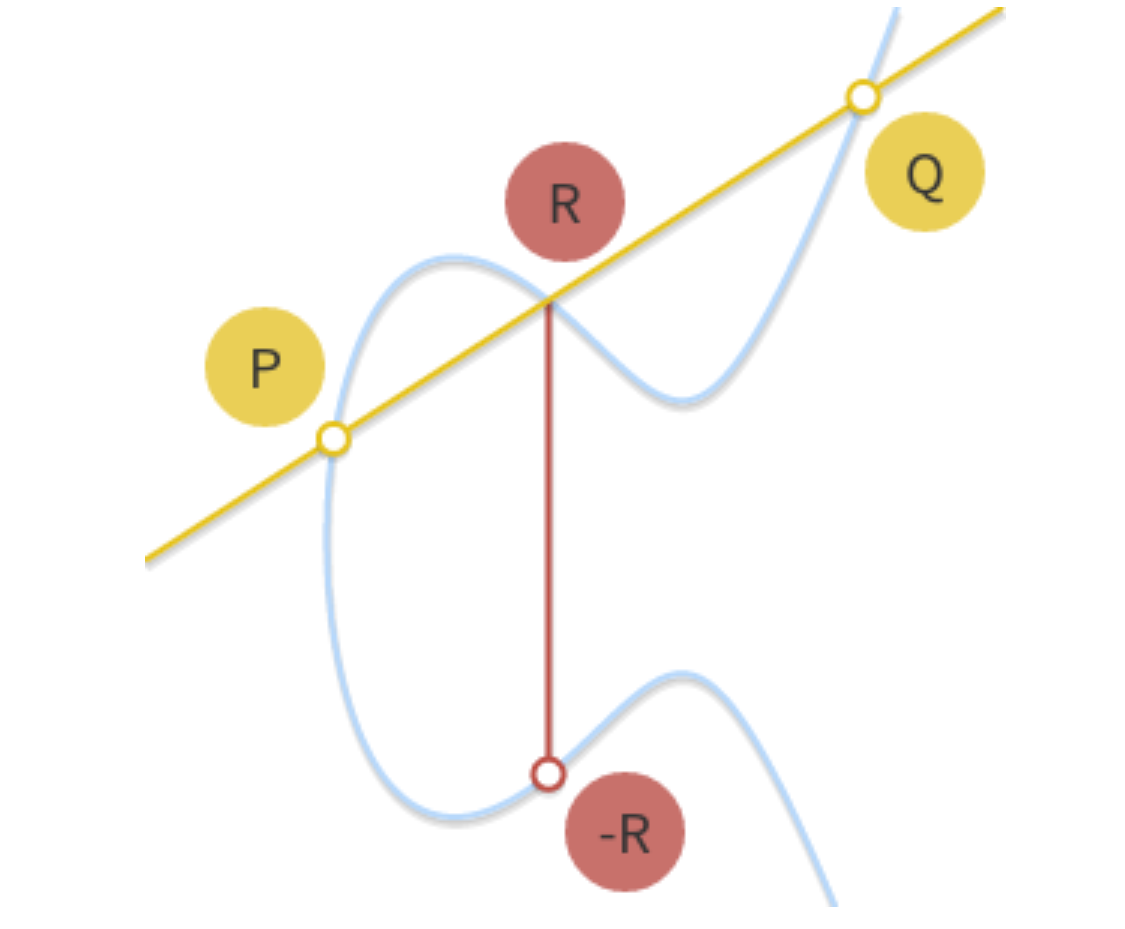
\includegraphics[scale=0.7]{add3.PNG}
    \item Here, P+Q=-R, and this is how ECC works (In case you would love to play with point adition and scalar multiplication using visual tool, here is one such thing - https://andrea.corbellini.name/ecc/interactive/reals-add.html 
    \item  And unsurprisingly, we can add one point to itself too \item How many steps would it take to compute x•P, where x is a random 256-bit integer? In this case, x can range anywhere from 0 to $1.1579209e+77$.
    It turns out that computing x•P would never require more than 510 point addition operations. Here’s why. First, compute the following series:
    $2^0•P, 2^1•P, 2^2•P, 2^3•P, 2^4•P, 2^{255}•P-1$
    \item We can define a group over elliptic curves where the elements of the group are the points of an elliptic curve;
    the identity element is the point at infinity 0;
    the inverse of a point $P$ is the one symmetric about the $x$-axis and addition is given by the following rule, that given three aligned non zero points $P,Q,R$, there sum is $P+Q+R=0$
    \item If we actually need to do something, we need to turn this geometric method into an algebraic method, but actually it can be really tedious because it requires solving cubic equations, but it is also not computationally difficult or anything
    \item If we are given $P$ and $n$, we have at least one polynomial time algorithm for computing $Q=nP$, but if we are given $Q$ and $P$ can we define $n$?This is known as logarithm problem. If we play with scalar multiplication for quite a while, we will even see some patterns from which we might think that we can come up with an algorithm which can solve this task. But there is a variant of this logarithm problem known as discrete logarithm problem, where we will see that if we reduce the domain of elliptic curves, the scalar multiplication still remains easy but discrete log become really a hard problem
\end{itemize}
\section{Elliptic Curves in $F_p$}
As a refresher, in fields we have two binary operations: addition (+) and multiplication (·). Both are closed, associative and commutative. For both operations, there exist a unique identity element, and for every element there's a unique inverse element. Finally, multiplication is distributive over the addition, $x.(y+z)=x.y+x.z$
From earlier intro, we actually defined elliptic curves as  $\begin{array}{rcl}
  \left\{(x, y) \in \mathbb{R}^2 \right. & \left. | \right. & \left. y^2 = x^3 + ax + b, \right. \\
  & & \left. 4a^3 + 27b^2 \ne 0\right\}\ \cup\ \left\{0\right\}
\end{array}$\\
Since we have restricted elliptic curves to finite fields, now we will say, \\
$\begin{array}{rcl}
  \left\{(x, y) \in (\mathbb{F}_p)^2 \right. & \left. | \right. & \left. y^2 \equiv x^3 + ax + b \pmod{p}, \right. \\
  & & \left. 4a^3 + 27b^2 \not\equiv 0 \pmod{p}\right\}\ \cup\ \left\{0\right\}
\end{array}$ where 0(or the identity element) is still the point at infinity, and $a$ and $b$  are two integers $F_p$, So what previously was a continuous curve is now a set of disjoint points in the $xy$-plane. Even if we have restricted our domain, elliptic curves in still form an abelian group. When it comes to point addition, clearly we need to change a bit our definition of addition in order to make it work in $F_p$. We can informally say that a line in $F_p$ is the set of points satisfying $ax+by+c=0(mod p)$.

The order of an elliptic curve group is the number of points in a group and we can find that using a fairly efficient algorithm (Schoof's algorithm)

\section{Scalar Multiplication and Cyclic Subgroups}
Multiplication over points for elliptic curves in $F_p$ has an interesting property. Take the curve $y^2 \equiv x^3 + 2x + 3 \pmod{97}$ and a point $P=(3,6)$. If we calculate the multiples of $p$, 
\begin{itemize}
    \item $0P=0$
    \item $1P=(3,6)$
    \item $2P=(80,10)$
    \item $3P=(80,87)$
    \item $4P=(3,91)$
    \item $5P=0$
    \item $6P=(3,6)$ and so on
\end{itemize}
    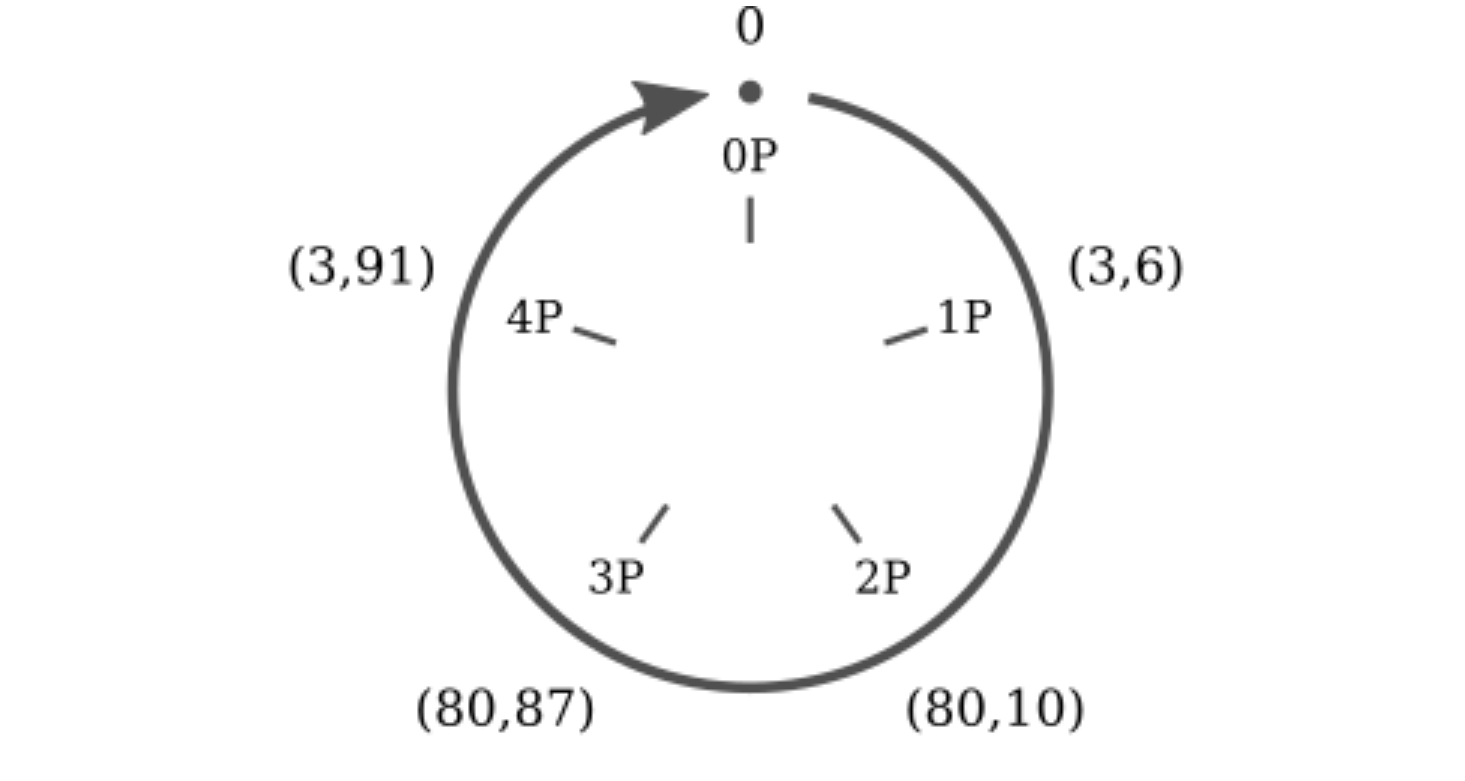
\includegraphics[scale=0.8]{add2.PNG}\\
We can immediately see two things: firstly, the multiples of  are just five: the other points of the elliptic curve never appear. Secondly, they are repeating cyclically and we can write $kP = (k \bmod{5})P$ and the point $P$ is called generator or base point of the cyclic subgroup.

Now the next thing immediately appearing in our mind is what is the order of the sub group generated by point $P$ and how we find that. Apparently, Schoof's algorithm can't be applied directly but we can take help from it sure :) In fact the order of a sub group generated by $P$ is the smallest $n$ such that $nP=0$, in above example which is $5$ and the order of $P$ is linked to the order of EC according to Lagrange's theorem, which states that the order of a subgroup is a divisor of the order of the parent group. In other words, if an elliptic curve contains $N$ points and one of its sub group contains $n$ points, then $n|N$. So these two information helps us find an obvious way to figure out such an $n$ yayy :D 
\section{But what is a good base point!?}
For our ECC algorithms, we want subgroups with a high order. So in general we will choose an elliptic curve, calculate its order $N$, choose a high divisor as the subgroup order $n$ and find a suitable base point. So we do not find a base point and then find its order, it's the other way around.

Oops but we need to define one more thing: co factor. Lagrange's theorem implies that the number $h=\frac{N}{n}$ is always an integer (because $n$ is a divisor of $N$). The number $h$ has a name: it's the co-factor of the subgroup.
Since for every point on the EC, we have $NP=0$, we can write $n(hP)=0$. Now say, $G=hP$, then if $n$ is prime, apparently, $G$ creates a sub group of order $n$(except when $G=hP=0$)
\section{Back to Discrete Logarithm}
We defined this problem earlier. Interestingly, it is *hard* that because is no known polynomial time algorithm for this problem. What makes ECC interesting is that, as of today, the discrete logarithm problem for elliptic curves seems to be "harder" if compared to other similar problems used in cryptography. This implies that we need fewer bits to achieve the same level of security as with other cryptosystems.

\section{Domain Parameters}
Our elliptic curve algorithms will work in a cyclic subgroup of an elliptic curve over a finite field. So we need $6$ different parameters, prime $p$ specifying the size of the field, co efficient $a$ and $b$, base point $G$, order $n$ of the sub group, co factor $h$ of the sub group.
\section{Are All Curves Good}
There are some classes of elliptic curves which are weak and allow the use of special purpose algorithms to solve the discrete logarithm problem efficiently. For example, all the curves that have $p=hn$ (when the order of the finite field is equal to the order of the elliptic curve) are vulnerable to Smart's attack, which can be used to solve discrete logarithms in polynomial time on a classical computer.

Now, if anyone gives you the domain parameters of a curve. there's the possibility that provider has discovered a new class of weak curves that nobody knows and built a "fast" algorithm for computing discrete logarithms on the curve provider gave you. How can the provider convinces you of the contrary, that it is not aware of any vulnerability?

To solve this kind of problem, sometimes we have an additional domain parameter: the seed $S$. This is a random number used to generate the coefficients $a$ and $b$, or the base point $G$, or both. These parameters are generated by computing the hash of the seed $S$. Hashes, as we know, are "easy" to compute, but "hard" to reverse.\\
$S= random()\\
 H = hash(S)\\
 a = f(H)\\
 b = g(H)$\\
 If we wanted to cheat and try to construct a seed from the domain parameters, we would have to solve a "hard" problem: hash inversion.
 
 \section{Elliptic Curve Cryptography}
Poof! We are finally here!
\begin{itemize}
    \item The private key is a random integer $d$ chosen from $\{1,2,\dots n-1\}$  (where $n$ is the order of the subgroup).
    \item The public key is the point $H=dG$ (where $G$ is the base point of the subgroup)
\end{itemize}
\section{Encryption with ECDH}
It is actually a key-agreement protocol, more than an encryption algorithm. This basically means that ECDH defines (to some extent) how keys should be generated and exchanged between parties. How we encrypt data using such keys is up to us.

The problem it solves is the following: two parties (the usual Alice and Bob) want to exchange information securely, so that a third party (M) may intercept them, but may not decode them. 

Here is how it works -
\begin{itemize}
    \item Alice and Bob generate their own private and public keys. We have the private key $d_A$ and the public key $H_A=d_AG$ for Alice, and the keys $d_B$  and $H_B=d_BG$ for Bob. Note that both Alice and Bob are using the same domain parameters: the same base point on the same elliptic curve on the same finite field.
    \item Alice and Bob exchange their public keys $H_A$  and $H_B$ over an insecure channel. M would intercept $H_A$ and $H_B$, but won't be able to find out neither $d_A$ nor $d_B$ without solving the discrete logarithm problem.
    \item Alice calculates $S=d_AH_B$ (using her own private key and Bob's public key), and Bob calculates $S=d_BH_A$ and clearly $S$ is the same for both
\end{itemize}
Now the question if M can infer anything about $S$ given $G$, $H_A$ and $H_B$. This is in fact The Diffie-Hellman problem for elliptic curves is assumed to be a "hard" problem. It is believed to be as "hard" as the discrete logarithm problem, although no mathematical proofs are available.
\section{Signing with ECDSA}
The scenario is the following: Alice wants to sign a message with her private key ($d_A$), and Bob wants to validate the signature using Alice's public key ($H_A$). Nobody but Alice should be able to produce valid signatures. Everyone should be able to check signatures.
ECDSA works on the hash of the message than on the message itself, but the hash needs to cryptographically secure. The hash of the message needs to be truncated so that the bit length of the hash is the same as the bit length of $n$ (the order of the subgroup). The truncated hash is an integer and will be denoted as $z$. 
The algorithm Alice uses for signing is the following- 
\begin{itemize}
    \item Take a random integer $k$ chosen from $\{1,2,\dots n-1\}$ (where $n$ is the subgroup order).
    \item calculate $P=kG$, $G$ being the base point of the subgroup
    \item Calculate $r = x_P \bmod{n}$, $x_P$ is the $x$ co ordinate of $P$, if $r=0$ then try again
    \item Calculate $s = k^{-1} (z + rd_A) \bmod{n}$, if $s=0$ then try again
\end{itemize}
\section{Verifying Signatures}
In order to verify the signature we'll need Alice's public key$H_A$, the (truncated) hash $z$ and, obviously, the signature $(r,s)$.
\begin{itemize}
    \item Calculate $u_1 = s^{-1} z \bmod{n}$
    \item Calculate $u_2 = s^{-1} r \bmod{n}$
    \item Calculate $P = u_1 G + u_2 H_A$
\end{itemize}
Now find $x_P$ and the sign is valid iff $r = x_P \bmod{n}$
\section{Correctness of the Algorithm}
In order to know whether this is correct, we just need to make sure that the point P in verifying signature part is the same as the signature generation algorithm.
We can write:\\
\begin{align*}
  P & = u_1 G + u_2 H_A \\
    & = u_1 G + u_2 d_A G \\
    & = (u_1 + u_2 d_A) G
\end{align*}
Using the definition from above, we can further write
\begin{align*}
  P & = (u_1 + u_2 d_A) G \\
    & = (s^{-1} z + s^{-1} r d_A) G \\
    & = s^{-1} (z + r d_A) G
\end{align*}
We know $s = k^{-1} (z + rd_A) \bmod{n}$. Modifying we can get $k = s^{-1} (z + rd_A) \bmod{n}$. Substituting the result in the equation, \begin{align*}
  P & = s^{-1} (z + r d_A) G \\
    & = k G
\end{align*}
Exactly what we have expected !
\section{What $k$ to choose}
We need to make sure that $k$s we are generating are really from a good *random* number generator and truly random.
If we use the same $k$ for all signatures, or if our random number generator were somewhat predictable, an attacker would be able to find out the private key and he would just need two signatures for that, say $(r_1,s_1)$ and $(r_2,s_2)$
together with the domain parameters, which will be the same and in fact $k$ is the same here. 
\begin{itemize}
    \item Note that $r_1 = r_2$ because $P_1=kG=P_2$ and $r = x_P \bmod{n}$ 
    \item $(s_1 - s_2) \bmod{n} = k^{-1} (z_1 - z_2) \bmod{n}$, this equation follows directly from the equation of $s$
    \item Rearranging, we get $k = (z_1 - z_2)(s_1 - s_2)^{-1} \bmod{n}$
\end{itemize}
Now we can find the value of the private key $d$ from the equations introduced before, $s = k^{-1}(z + rd) \bmod{n}\ \ \Rightarrow\ \ d = r^{-1} (sk - z) \bmod{n}$ 
\section{Let's Break Discrete Logarithm Problem}
As a fresher, given two points $P$ and $Q$,find out the integer $x$ that satisfies the equation $Q=xP$. The points belong to a subgroup of an elliptic curve, which has a base point $G$ and whose order is $n$.
\subsection{Baby Step Giant Step Algorithm}
We can write any integer $x$ such that $x=am+b$. So we can say:
\begin{align*}
  Q & = xP \\
  Q & = (am + b) P \\
  Q & = am P + b P \\
  Q - am P & = b P
\end{align*}
The algorithm is the following - 
\begin{itemize}
    \item Calculate $m = \left\lceil{\sqrt{n}}\right\rceil$
    \item For every b in $0,1,\dots m$ calculate $bP$ and store the result in a hash table
    \item For every a in $0,1,2\dots m$:
    \begin{itemize}
        \item Calculate $amP$
        \item Calculate $Q-amP$
        \item Check the hash table to see if there exists a point $bP$ such that $Q-amP=bP$
    \end{itemize}
\end{itemize}
If we look at what this algorithm is doing, we will see that when $a=0$, we have been checking whether $Q$ is among $0P$ to $mP$, when $a=1$, we are checking whether $Q$ is among $mP$ to $2mP$ and so on and this way finally from $(m-1)P$ to $m^2P$ or roughly $nP$.

Since look up takes constant time, the algorithm has both time and space complexity $O(\sqrt{n})$ or $O(2^{k/2})$, if you consider that $n$ has $k$ bits. Now let's try to see how huge this number is :')

Let's take a standardized curve: prime192v1 (aka secp192r1, ansiX9p192r1). This curve has order $n=0xffffffffffffffff ffffffff99def836146bc9b1\\b4d22831$.Suppose each point needs exactly 32 bytes: our hash table would need approximately $2.5*10^{30}$ bytes of memory. Looking on the web, it seems that the total world storage capacity is in the order of the zettabyte ($10^{21}$ bytes). Imagine trying to store this thing poof :(
\subsection{Pollard's $\rho$}
Here we attempt to solve a slightly different problem, when we are asked to find $x$ given that $Q=xP$, we try to solve given $Q,P$ can we find $a,b,A,B$ such that $aP+bQ=AP+BQ$
If we find such four things, we can write- 
\begin{align*}
  aP + bQ & = AP + BQ \\
  aP + bxP & = AP + BxP \\
  (a + bx) P & = (A + Bx) P \\
  (a - A) P & = (B - b) xP
\end{align*}
We can get rid of $P$. Recall that our subgroup is cyclic with order $n$, so we can write -
\begin{align*}
  a - A & \equiv (B - b) x \pmod{n} \\
  x & = (a - A)(B - b)^{-1} \bmod{n}
\end{align*}
Now how to find $a,b,A,B$? The principle of operation of Pollard's rho is simple: we generate a pseudo-random sequence of points $X_1,X_2,\dots$ where each $X_i=a_iP+b_iQ$ The sequence can be generated using a pseudo-random function $f$ like this:\\
$(a_{i + 1}, b_{i + 1}) = f(X_i)$\\
It doesn't really matter how $f$ works internally (although certain functions may yield results faster than others), what matters is that $f$ determines the next point in the sequence based on the previous one, and that all the $a_i$ and $b_i$ coefficients are known by us.
By using such $f$, sooner or later we will see a loop in our sequence. That is, we will see a point $X_j=X_i$.The reason why we must see the cycle is simple: the number of points is finite, hence they must repeat sooner or later. Once we see where the cycle is, we can use the equations above to figure out the discrete logarithm. Now how to detect cycle efficiently?
\subsubsection{Tortoise and Hare Algorithm}
The main idea is that We take two pets, the tortoise and the hare, and make them walk our sequence of points from left to right. The tortoise is slow and reads each point one by one; the hare is fast and skips a point at every step. After some time both the tortoise and the hare will have found the same point, but with different coefficient pairs. Or, to express that with equations, the tortoise will have found a pair $(a,b)$ and the hare will have found a pair $(A,B)$ such that $aP + bQ = AP + BQ$.

It's easy to see that this algorithm requires constant memory. Calculating the asymptotic time complexity is not that easy, but a probabilistic proof that shows how the time complexity is $O(\sqrt{n})$ as we have already said. The proof is based on the "birthday paradox", which is about the probability of two people having the same birthday.

Now since this is good on the aspect of space, let's consider how much it would take to break it. As we have already said, prime192v1 is one of the "smallest" elliptic curves(Has the smallest order among standardized curves). We also said that Pollard's $\rho$ has  time complexity $O(\sqrt{n})$. If we used the same technique as Chris Monico(who used the parallelized version of pollard's $rho$ to break $109$ bit long curve and that took $17$ months calendar time) (the same algorithm, on the same hardware, with the same number of machines), how much would it take to compute a logarithm on prime192v1?
$17\ \text{months}\ \times \frac{\sqrt{2^{192}}}{\sqrt{2^{109}}} \approx 5 \cdot 10^{13}\ \text{months}$
\section{Tomorrow's Techniques}
\subsection{Shor's Algorithm}
Tomorrow's techniques are a bit more worrisome: there exists a quantum algorithm capable of computing discrete logarithms in polynomial time: Shor's algorithm, which has time complexity $O((\log n)^3)$ and space complexity $O(\log n)$

Quantum computers are still not sophisticated enough to run algorithms like Shor's, still the need for quantum-resistant algorithms may be something worth investigating now. What we encrypt today might not be safe tomorrow.
\section{Why ECC}
Long story short, in order to achieve the same level of security ECC requires way less number of bits than RSA and smol things are easy to maintain :')
\section{Where does ECC come into play}
Yes we require for it zkSNARK. We will not introduce zkSNARK here, rather we will dive deep into how ECC and elliptic curve pairing comes into play in zkSNARK\\
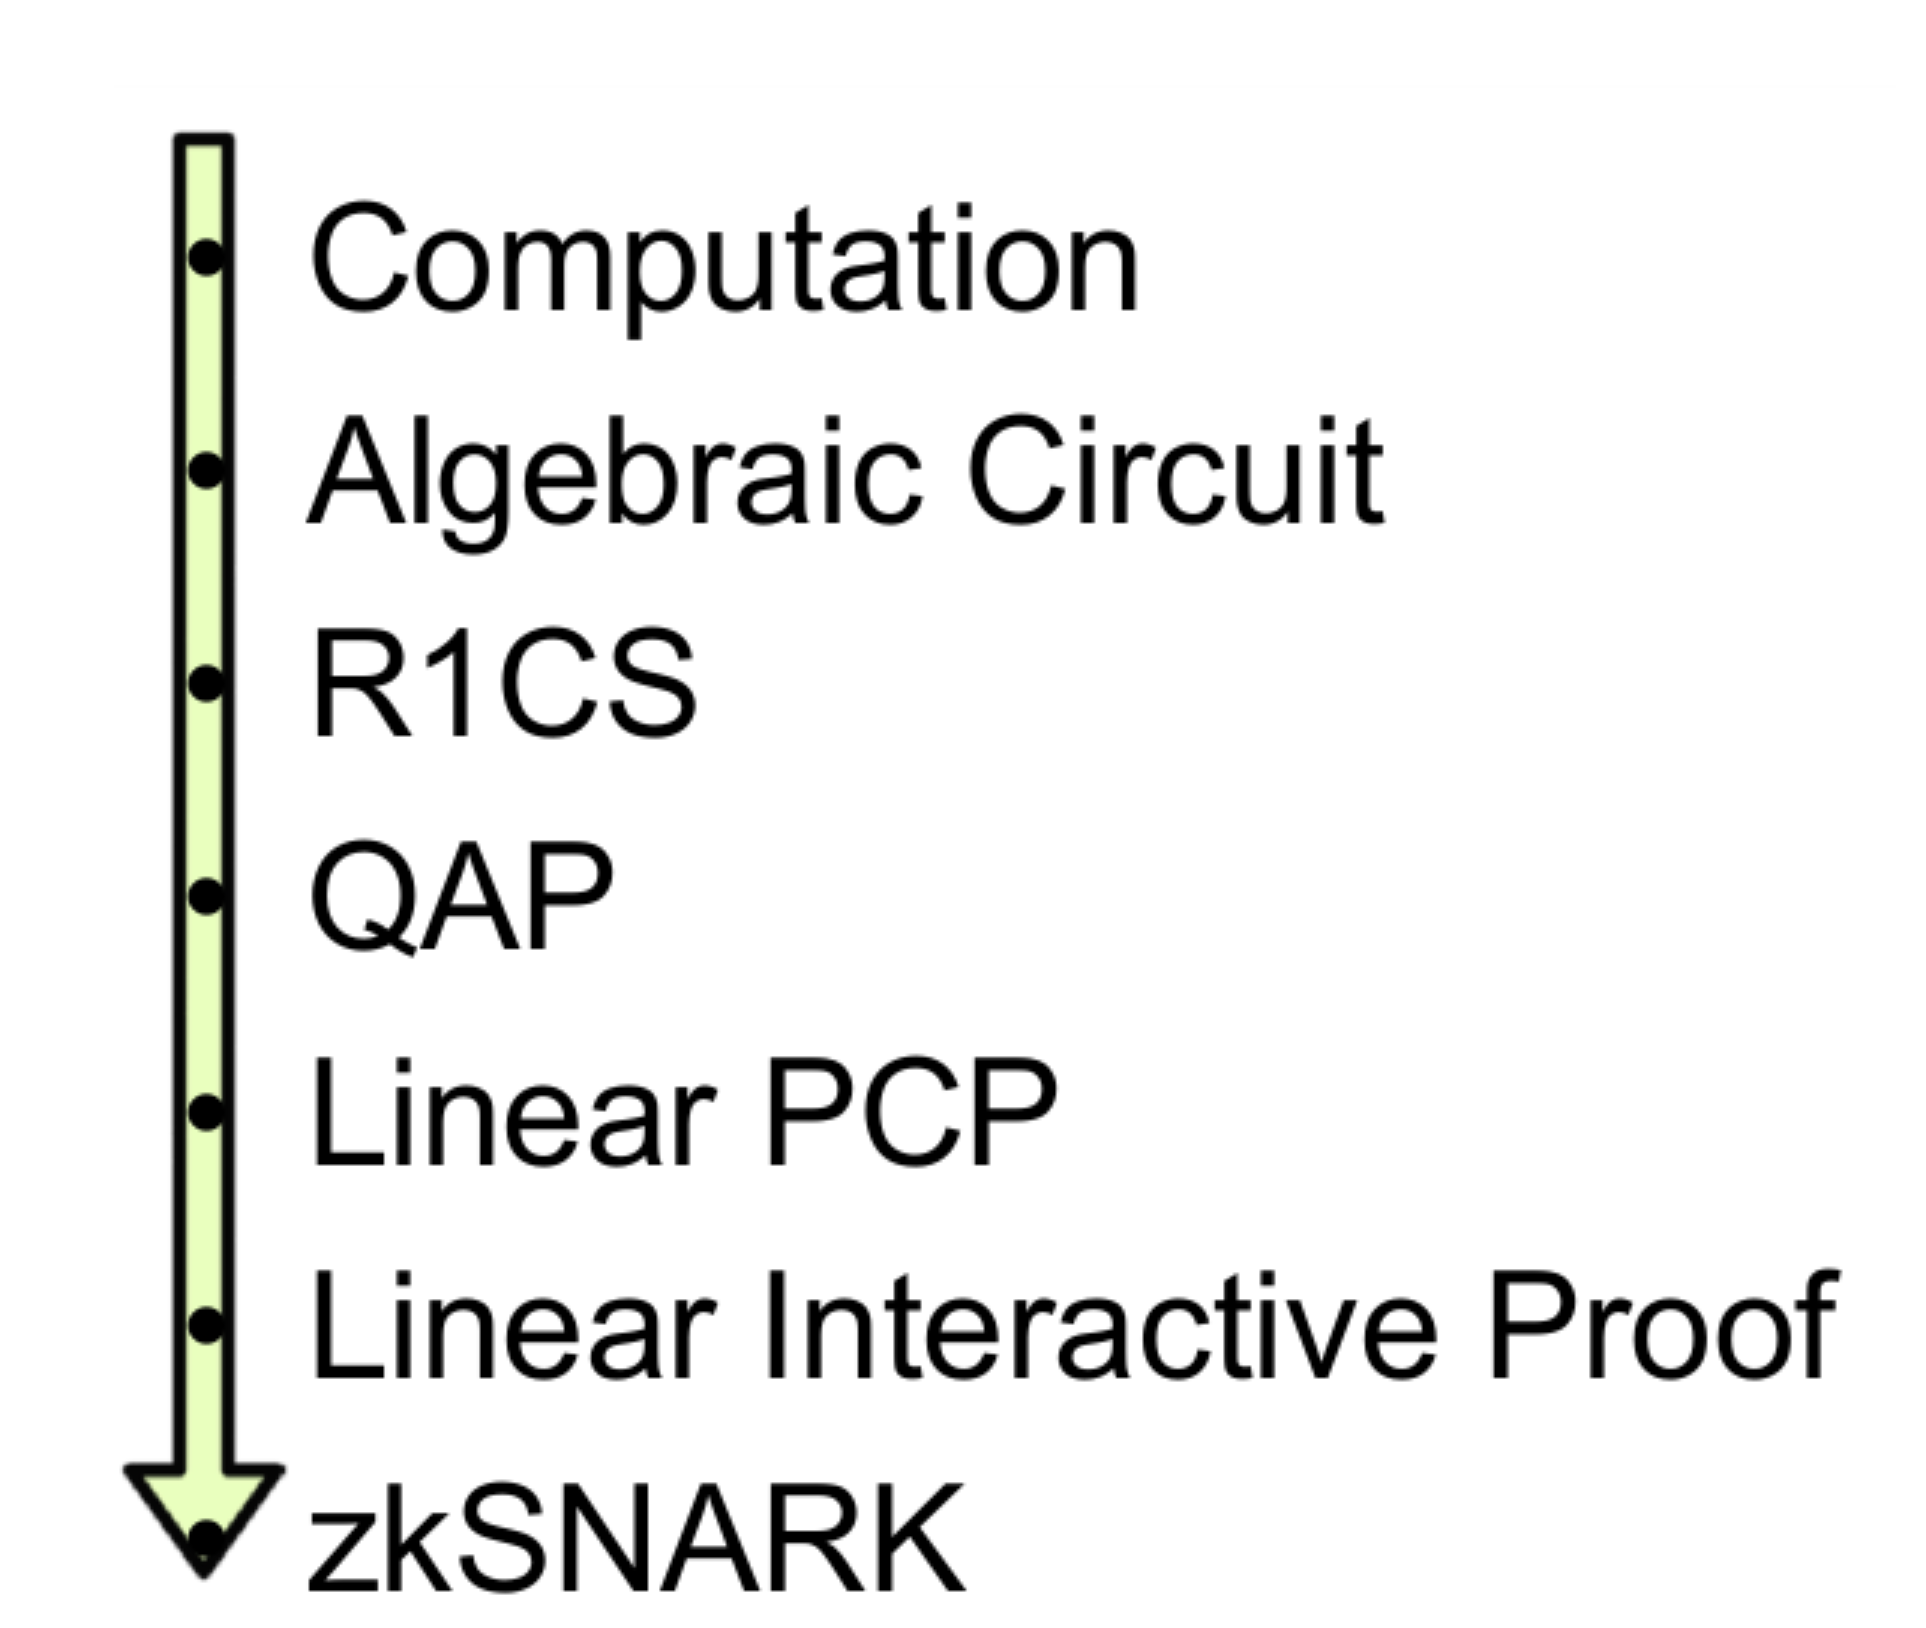
\includegraphics[scale=0.7]{Eren.PNG}\\
This is the first half of the pipeline drawn by zkSNARK researcher Eran Tromer. Since zk-SNARKs cannot be applied to any computational problem directly; we will have to convert the problem into the right “form” for the problem to operate on. The form is called a “quadratic arithmetic program” (QAP). This article will eventually dive deeper into as many aspects as it can, for the time being we will discuss about QAP and how it comes into play, we will eventually discuss about trusted setup and multi party computation too, so sit tight :DD 
\section{QAP}
The example we will play here is $x^3+x^2+4=84$. You are a prover and you want to prove that you know this solution to this equation. We have 3 main steps here- flattening, conversion to R1CS(rank 1 constraint system) and finally R1CS to QAP. The goal of code flattening is to convert the original code, which may contain arbitrarily complex statements and expressions, into a sequence of statements that are of two forms:
\begin{itemize}
    \item $x=y$ (where $y$ can be a variable or a number)
    \item $x= y (op) z$ where $op\in\{+,-,*,/\}$ and $y$ and $z$ are variables
\end{itemize}
\subsection{Flattening}
So following the above rules, the results of the flattening process for our equation is as follows-
\begin{itemize}
    \item  $v_1 = x*x$
    \item  $v_2 = v_1*x$
    \item  $v_3 = v_1 + v_2$
    \item  $out = v_3 + 4$
\end{itemize}
\subsection{Gates to R1CS}
Now we convert them into rank 1 constraint system(R1CS). An R1CS is a list of triplets of three vectors

$(\vec{a_i},\vec{b_i},\vec{c_i})$, and the solution to an R1CS is a vector $\Vec{s}$, where $\vec{s}$ must satisfy the equation $\langle \vec{a_i}, \vec{s} \rangle \ast \langle \vec{b_i}, \vec{s} \rangle - \langle \vec{c_i}, \vec{s} \rangle = 0 \quad \textrm{for} \quad \forall i\\$
The triplets can be interpreted as defining constraints, which need to be satisfied by finding $\vec{s}$ such that the equations above hold. To transform the flattened version of our code to a R1CS, first we define a vector, which will hold the state of our program, i.e. all variables which are used in the program. Each component of this vector will be one variable and the solution $\vec{s}$ will be an assignment to each variable.
$
\vec{s} = \begin{pmatrix} 
1 \\ 
x \\ 
v_1 \\ 
v_2 \\
v_3 \\
out
\end{pmatrix}
$
We will soon see why we have to put $1$ in $\vec{s}$, it is to deal with constants.
For example, to encode the first line in the function body we can set:\\
\begin{itemize}
    \item $\vec{a_1}=(0,1,0,0,0,0)$
    \item $\vec{b_1}=(0,1,0,0,0,0)$
    \item $\vec{c_1}=(0,0,1,0,0,0)$
\end{itemize}
Let's check the expansion of this line-\\
\begin{equation} 
\langle \vec{a_1}, \vec{s} \rangle \ast \langle \vec{b_1}, \vec{s} \rangle - \langle \vec{c_1}, \vec{s} \rangle = \sum_{i=1}^{n} a_{1,i} s_i \ast \sum_{i=1}^{n} b_{1,i} s_i - \sum_{i=1}^{n} c_{1,i} s_i = x \ast x - v_1 = 0 
\end{equation}
To encode the second line, we can set:
\begin{itemize}
    \item $\vec{a_2}=(0,1,0,0,0,0)$
    \item $\vec{b_2}=(0,0,1,0,0,0)$
    \item $\vec{c_2}=(0,0,1,1,0,0)$
\end{itemize}
And we can verify,
\begin{equation} 
\langle \vec{a_2}, \vec{s} \rangle \ast \langle \vec{b_2}, \vec{s} \rangle - \langle \vec{c_2}, \vec{s} \rangle = \sum_{i=1}^{n} a_{2,i} s_i \ast \sum_{i=1}^{n} b_{2,i} s_i - \sum_{i=1}^{n} c_{2,i} s_i = x \ast v_1 - v_2 = 0 
\end{equation}
We can complete the third and fourth equations in the same way - \begin{itemize}
    \item $\vec{a_3}=(0,0,1,1,0,0)$
    \item $\vec{b_3}=(1,0,0,0,0,0)$
    \item $\vec{c_3}=(0,0,0,0,1,0)$
\end{itemize}
Now we can see what role $1$ plays in addition check. We will o ahead and do the final one.
\begin{itemize}
    \item $\vec{a_4}=(4,0,0,0,1,0)$
    \item $\vec{b_4}=(1,0,0,0,0,0)$
    \item $\vec{c_4}=(0,0,0,0,0,1)$    
\end{itemize}
Thus we have our R1CS with $4$ constraints. The witness is the assignment to all the variables, including input, output and internal variables. (Will add my experience here, when it was the first time of my trying to implement a zkSNARK circuit, everything was going above my head, by now I was able to connect all the dots as I continued working on this article and everything makes so much sense and it is just so rewarding) 
$[1,4,16,64,80,84]$
\subsection{R1CS to QAP}
To complete the transformation to a QAP we need to switch from vectors to polynomials. We start by defining polynomials $A_i(x),B_i(x),C_i(x)$ for $i\in [1,N]$ when $N$ is the number of elements in any of the constraint vectors, in our case this is $6$. Then we construct polynomials that satisfy this $A_i(n)=\vec{a_{n,i}}$ and same goes for all $B_i$s and $C_i$s and it is obvious to see that $n$ must be $4$ leading to the conclusion that each $A_i,B_i,C_i$ will be a polynomial of degree $4$ and we have each of these polynomials evaluated at $4$ points, we can find the polynomials using lagrenge interpolation, we won't go into details here.With these definitions we can now express the R1CS from above as one equation $A(x) \ast B(x) - C(x) = H(x) \ast Z(x)$ where \\
$\vec{A(x)}= \begin{pmatrix} 
A_1(x) \ 
A_2(x) \ 
A_3(x) \ 
A_4(x) \
A_5(x) \ 
A_6(x)
\end{pmatrix}$\\
$\vec{B(x)}= \begin{pmatrix} 
B_1(x) \ 
B_2(x) \ 
B_3(x) \ 
B_4(x) \ 
B_5(x) \ 
B_6(x)
\end{pmatrix}$\\
$\vec{C(x)}= \begin{pmatrix} 
C_1(x) \ 
C_2(x) \ 
C_3(x) \ 
C_4(x) \ 
C_5(x) \ 
C_6(x)
\end{pmatrix}$\\
$A(x) = \langle \vec{A},\vec{s} \rangle$\\
$B(x) = \langle \vec{B},\vec{s} \rangle$\\
$C(x) = \langle \vec{C},\vec{s} \rangle$\\
$Z(x) = (x - 1)(x - 2)(x - 3)(x - 4)$\\
Let's try to see what all these means. Note that by definition, $\vec{A(1)} = \vec{a_1}$,$\vec{A(2)} = \vec{a_2}$,$\vec{A(3)} = \vec{a_3}$,$\vec{A(4)} = \vec{a_4}$ and the same goes for $\vec{B(x)}$ and $\vec{C(x)}$ and combining all these definitions, we can say that R1CS is equivalent to \\
$A(x) \ast B(x) - C(x) = 0 \quad \textrm{for} \quad x \in \{1,2,3,4\}$ and this can happen if \\
$\exists H(x): A(x) \ast B(x) - C(x) = H(x)(x-1)(x-2)(x-3)(x-4)$ and It must be the prover who will compute $\vec{H(x)}$ because this shows that the prover knows a satisfying assignment $\vec{s}$ to the underlying R1CS.

I will mention one important idea which will come in handy afterwards and that is evaluating polynomial at hidden points,without actually knowing the point! Does anything come in your mind regarding how we can go about it?

If you have another function that has *good* behavior, like linear, injective and one way(this means if this function being evaluated at $x$ gives $z$, it is hard for you to generate $x$ given $z$), then this function can help you out!!

Here is how: imagine I want you to evaluate a polynomial of $x_0$ at such function $f$, so I want you to find $f(P(x_0))$ without giving away the value of $x_0$ where $P(x)$ is a $d$ degree polynomial. What can I do?

I can send you $f(1), f(x_0), f(x_0^2), \cdots, f(x_0^d)$ because then you can compute, $
f(P(x_0)) = f(a_0 + a_1 x_0 + \cdots + a_n x_0^d)\\
= f(a_0) + f(a_1 x_0) + \cdots + f(a_d x_0^d) \\
= a_0 f(1) + a_1 f(x_0) + \cdots + a_d f(x_0^d) 
$
Observe that we have used the properties mentioned earlier, for which you cannot reverse engineer the values the function $f$ was evaluated on and we also used the linearity. 

This is the end of section QAP. We are going to talk about elliptic curve pairing next(but before that we will take a look into where we are currently now and what we are trying to do), it honestly requires so much formal math which I won't dive deep into here, but I will still give a higher level of technical detail of how things work in pairing. 

\section{Where are we now!?}
In case you feel lost about what am I trying to do, I will remind you of our goals, I want to give the understanding of zkSNARK in as depth as possible and demystify everything. ZKSNARKs are impressive, you can verify the correctness of computations without having to execute them and you will not even learn what was executed - just that it was done correctly. Current zkSNARKs have $4$ main components- 
\begin{itemize}
    \item Encoding as o polynomial problem, which we explained in the earlier section and the program which we are gonna check will be converted to a quadratic equation of polynomials as we showed before where the equality holds if and only if the program is computed correctly and the prover wants to convince the verifier that this equality holds.
    \item succinctness, the verifier chooses a secret evaluation point s to reduce the problem from multiplying polynomials and verifying polynomial function equality to simple multiplication and equality check on numbers, $t(s)h(s) = w(s)v(s)$, which significantly increases the computational efficiency and reduces the time so much
    \item Homomorphic encryption/ decryption, an encryption function E is used that has some homomorphic properties (but is not fully homomorphic, something that is not yet practical). This allows the prover to compute $E(t(s)), E(h(s)), E(w(s)), E(v(s))$ without knowing $s$, but they know $E(s)$ and some other helpful values. ECC we introduced in detail beforehand is used for this part, we will soon show more details once introduce pairing
    \item Zero knowledge, The higher level idea is that checking $t(s)h(s) = w(s)v(s)$ is identical to checking $t(s)h(s) k = w(s)v(s)k$ for a non zero random secret number $k$,but what makes difference is that if you are sent only the numbers $(t(s)h(s) k)$ and $(w(s)v(s) k)$, it is impossible to derive $t(s)h(s)$ or $w(s)v(s)$.
\end{itemize}
Now since now we are reminded of our goal, we can move to the next section.
\section{Elliptic Curve Pairing}
We will introduce a new operator $e(P,Q)$ here, it has very notation heavy formal definition which I will not introduce here, but basically this is a bilinear map, so it satisfies these constraints - 
\begin{itemize}
    \item $e(P, Q + R) = e(P, Q) * e(P, R)$
    \item $e(P + S, Q) = e(P, Q) * e(S, Q)$
\end{itemize}
One very important thing here is that $+$ and $*$ can be arbitrary;how $+$ and $*$ are defined is not important as long as they are consistent in the usual ways, eg. $a + b = b + a, (a * b) * c = a * (b * c)$ and $(a * c) + (b * c) = (a + b) * c$. An elliptic curve pairing is a function that takes a pair of points on an elliptic curve and returns an element of some other group, called the target group. For some $g_1$, $g_2$, and $g_3$ on the curve and integers $a$ and $b$, these properties are satisfied(and why so we can infer from earlier bilinear mapping properties - 
\begin{itemize}
    \item $e(a*g_1,g_2)=e(g_1,g_2)^a$
    \item $e(g_1,b*g_2)=e(g_1,g_2)^b$
    \item $e(g_1+g_2,g_3)=e(g_1,g_3)*e(g_2,g_3)$
    \item $e(g_1,g_2+g_3)=e(g_1,g_2)*e(g_1,g_3)$
\end{itemize}
Also a pairing needs to have another property named non-degeneracy and it says $e(g_1,g_2)\ne 1$ and efficient computability, for example, we can make an easy pairing by simply taking the discrete logarithms of all points and multiplying them together, but this is as computationally hard as breaking elliptic curve cryptography in the first place and we do not count on it. How elliptic curve pairing works require really advanced algebra, introducing them might deviate from our goal, so we won't do that here, but I think introducing to the meat of it might be a good thing since once you really like something, you would really love going deeper about it. 

Now we will give an essence of how it is used in zkSNARK. Suppose I want to convince you that I know an integer solution to $x^2-5x+6=0$ but I won't reveal it. What I can do is I can take my root $a$ and a pair of elliptic curves $g_1$ and $g_2$ and send you $a*g_1$ and $a*g_2$ along with $g_1$ and $g_2$. As we discussed earlier, looking at these points, it will be computationally infeasible for you to find out $a$ (ECDLP). Now you can take a pairing and compute $e(a*g_1,a*g_2)e(g_1,-5*ag_2)e(6*g_1,g_2)$ which is equal to $e(g_1,g_2)^{a^2-5a+6}$. Now if this equals $1$, you can infer that $a^2-5a+6=0$ with high probability. The non-degeneracy condition, along with a large target group ensures this. In a zk-SNARK, elliptic curve pairings are used to check a system of quadratic constraints in this way the system of constraints is converted into a single large polynomial(we devoted a section for that) that has particular roots only if each of the quadratic constraints is satisfied.
\section{Formal QAP and application to zkSNARK}
This section will assume that you have a basic understanding of complexity terms(like P,NP, NP HARD, NP COMPLETE etc). Due to the very celebrated proof $IP=PSPACE$(thanks to 18.404), we got to know arithmetization as a technique. Arithmetization of Boolean computations is a well known technique and it maps
a Boolean circuit to a set of polynomial (e.g., quadratic) equations over a field and QSPs(QAP is a variant of it) use a new approach to the well-known technique of arithmetization of Boolean circuits.

Earlier, we introduced a simplified QAP, in real life scenarios,the addition, multiplication, subtraction and division will happen not with regular numbers, but rather with finite field elements so all answers are elements of some finite-sized set, usually integers within the range from $0$ to $n-1$ for some $n$ so we do not need to worry about rounding errors and it allows the system to work nicely with elliptic curves.

We will now move to the formal definition of QAP since we will actually need it to do the zkSNARK thing. A QAP $Q$ over field $F$ of input length $n$ consists of - 
\begin{itemize}
    \item Three sets of polynomials $V=\{v_k(x),k \in \{0,1,\dots m\}\}$, $W=\{w_k(x),k \in \{0,1,\dots m\}\}$,$Y=\{y_k(x), k \in \{0,1,\dots m\}\}$ and a divisor polynomial $D(x)$ all from $F[x]$. If you recall what we did before, these are what we introduced as $A(x),B(x),C(x)$ and $Z(x)$ respectively :)
    \item $f: \left\{(i, j) |1\leq i \leq n, j\in{0,1} \right\} \to \left\{1, ... m\right\}$
\end{itemize}
And an input $u$ is accepted and verified by QAP if we have $a_1,a_2\dots a_m$, $b_1,b_2,\dots b_m$, $c_1,c_2,\dots c_m$ from the field $F$ such that $(V_0 (x) + \sum_{k = 1}^ {k=m}a_k\cdot v_k(x)) \cdot(w_0 (x) + \sum_{k = 1} ^{k= m}b_k\cdot w_k(x)) -(y_0(x)+\sum_{k = 1}^{k=m}c_k\cdot y_k (x))$ divides $D(x)$. Actually $a_i$s,$b_i$s,$c_i$s have also some other constraints related to $f$, but they do not have a vital role in understanding zkSNARK part, so we will omit it here. I think by now we should be able to relate this formal definition to the QAP part introduced in an earlier section.

So zkSNARK has two phases(If you start implementing zkSNARK circuit, it will be evident how these phases work together and now that I am writing this and simultaneously implemented one such circuit, everything feels so connected and engaging to me :)), one is a setup phase and another is a proof phase. From now on, we will simplify the earlier introduced QAP definition a little bit, we will say that $V_0 (x) + \sum_{k = 1}^ {k=m}a_k\cdot v_k(x)=V_a$,$w_0 (x) + \sum_{k = 1} ^{k= m}b_k\cdot w_k(x)=W_b$,$y_0(x)+\sum_{k = 1}^{k=m}c_k\cdot y_k (x)=Y_c$. We can already see is how to verify them much more efficiently, because the verification task consists of checking whether one polynomial divides another polynomial. This can be facilitated by the prover in providing another polynomial $H$ such that $D\cdot H=V_a\cdot W_b-Y_c$ in other words verifier has to check  $D\cdot H-V_a\cdot W_b+Y_c=0$, i.e. checking that a certain polynomial is the zero polynomial. This looks rather easy, but the polynomials used in real life scenarios are quite large (the degree is approx. $100$ times the number of gates in the original circuit) so that multiplying two polynomials is not easy.

So instead of actually computing $V_a,W_b,Y_c$ and their product, the verifier chooses a secret random point $s$ (this point is part of the “toxic waste” of zCash and we will have a section devoting to the discussion of toxic waste), computes the numbers $D(s)$, $v_k(s)$,$w_k(s)$,$y_k(s)$ for all $k$ and from them,computes  $V_a(s)$, $W_b(s)$, $Y_c(s)$ and only checks that $D(s)H(s) = V_a(s)W_b(s)-Y_c(s)$. So a bunch of polynomial additions, multiplications with a scalar and a polynomial product is simplified to field multiplications and additions.

In some earlier section we introduced how to evaluate polynomial succinctly and with zero knowledge. We will formalize the idea more here but will first look at a simpler case, namely just the encrypted evaluation of a polynomial at a secret point, and not the full QSP problem. For this, we fix a group (an elliptic curve is usually chosen) and a generator $g$. Remember that a group element is called generator if there is a number $n$ (the group order) such that the list $g^0, g^1, g^2, …, g^{n-1}$ contains all elements in the group. The encryption is simply $E(x)= g^x$. Now the verifier chooses a secret field element $s$ and publishes (as part of the CRS) $E(s^0), E(s^1),\cdots , E(s^d)$ - $d$ is the maximum degree of all polynomials. Using these values, the prover can compute $E(f(s))$ for arbitrary polynomial $f(s)$ without ever knowing $s$, we showed how to do so earlier.

Hold on, since $s$ was destroyed the verifier cannot check that the prover evaluated the polynomial correctly, so what he did is the following,he also choose another secret field element, $\alpha$, and publish the following “shifted” values:
$E(\alpha s^0), E(\alpha s^1), ..., E(\alpha s^d)$. $\alpha$ too is also destroyed and known neither to the prover nor to the verifier.Using these encrypted values, the prover can similarly compute $E(\alpha f(s))$,for exampls is $f(s)=4s^2+2s+4$ then this is\\
$E(4\alpha s^2 + 2\alpha s + 4\alpha)\\
=g^{\alpha(4s^2+2s+4)}= (g^{\alpha s^2})^4(g^{\alpha s})^2(g^\alpha)^4\\
= E(\alpha s^2)^4 E(\alpha s^1)^2 E(\alpha s^0)^4$. So the prover publishes $A=E(f(s))$ and $B=E(\alpha f(s))$ and the verifier can use a pairing function to verify this, the elliptic curve and $e$ has to be chosen together such that $e(g^x,g^y)=e(g,g)^{xy}$ holds for all $x,y$

Using the pairing function, the verifier can check whether $e(A,g^\alpha)=e(B,g)$, note that $g^\alpha$ is known to the prover because it is infact the case that $E(\alpha s^0)=g^\alpha$, In order to see that this check is valid if the prover does not cheat, let's see these equalities \\
$e(A,g^\alpha)=e(g^f(s),g^\alpha)=e(g,g)^{\alpha f(s)}$\\
$e(B,g)=e(g^{\alpha f(s)},g)=e(g,g)^{\alpha f(s)}$

Now we will define the SNARK for QAP problem. In the previous para, we explained how the common reference string (CRS) is set up. After choosing secret numbers $s$ and $\alpha$ we publish
\begin{itemize}
    \item $E(s^0), E(s^1), ... , E(s^d)$
    \item $E(\alpha s^0), E(\alpha s^1), ... , E(\alpha s^d)$
    \item $E(D(s)), E(\alpha D(s))$
    \item $E(v_0(s)), ... E(v_m(s)), E(\alpha v_0(s)), ..., E(\alpha v_m(s))$
    \item $E(w_0(s)), ... E(w_m(s)), E(\alpha w_0(s)), ..., E(\alpha w_m(s))$
    \item $E(y_0(s)), ... E(y_m(s)), E(\alpha y_0(s)), ..., E(\alpha y_m(s))$
\end{itemize}
And we need further secret numbers $\beta_v, \beta_w, \beta_y, \gamma $ (they will be used to verify that those polynomials were evaluated and not some arbitrary polynomials) and publish
\begin{itemize}
    \item $E(\gamma), E(\beta_v\gamma), E(\beta_w\gamma), E(\beta_y\gamma)$
    \item $E(\beta_vv_1(s)), ... , E(\beta_vv_m(s))$
    \item $E(\beta_ww_1(s)), ... , E(\beta_ww_m(s))$
    \item $E(\beta_yy_1(s)), ... , E(\beta_yy_m(s))$
    \item $E(\beta_vD(s)), E(\beta_wD(s)), E(\beta_yD(s))$
\end{itemize}
This is the full common reference string. In practical implementations, may be not all elements of the CRS are needed, but that would complicate the presentation, so putting everything here.

Now what does the prover do? She has to find the polynomial $h$ and the values $a_1,\cdots ,a_m,b_1, \cdots ,b_m$. In order to describe what the prover sends to the verifier as proof, we have to go back to the definition of the QSP. There was an injective function $f: \left\{(i, j) |1\leq i \leq n, j\in{0,1} \right\} \to \left\{1, ... m\right\}$ and this function controlled the values of $a_i$s and $b_i$s since $m$ is pretty large, there are numbers which do not appear in the output of $f$ for any input. These indices are not restricted, so let us call them $I_{free}$ and let's define $v_{free}(x) = \sum_k a_kv_k(x)$ where the $k$ ranges over all indices in $I_{free}$. 

Now our proof consists of the following - 
\begin{itemize}
    \item $V_{free} := E(v_{free}(s)), \ W := E(w(s)), \ Y := E(y(s)), \ H := E(h(s))$
    \item $V_{free}' := E(\alpha v_{free}(s)), W' := E(\alpha w(s)), Y' := E(\alpha y(s)), H' := E(\alpha h(s))$
    \item $P := E(\beta_vv_{free}(s) + \beta_ww(s) + \beta_yy(s))$
\end{itemize}
The last part is used to check that the correct polynomials were used. Now the verifier does the following - since the values of $a_k$, where $k$ is not a “free” index can be computed directly from the input $u$ (which is also known to the verifier, this is what is to be verified), the verifier can compute the missing part of the full sum for v:
$v_{in}(x) = \sum_k a_kv_k(x)$ where the $k$ ranges over all indices not in $I_{free}$.
The verifier now confirms the following equalities using the pairing function $e$
\begin{itemize}
    \item $e(V_{free}', g) = e(V_{free}, g^\alpha), e(W', E(1)) = e(W, E(\alpha)), e(Y', E(1)) = e(Y, E(\alpha)),\\
    e(H', E(1)) = e(H, E(\alpha))$
    \item $e(E(\gamma), P) = e(E(\beta_v\gamma), V_{free})e(E(\beta_w\gamma), W)e(E(\beta_y\gamma), Y)$
    \item $e(E(v_0(s))E(v_{in}(s))V_{free}, E(w_0(s))W) = e(H, E(D(s)))e(y_0(s)Y, E(1))$
\end{itemize}
Ah I know a lot is going on, but our technical parts are gonna end soon, like real soon :')
Okay let's try to understand what are they doing, recalling from the section about evaluating polynomials at secret points, the first four conditions basically verify that the prover did evaluate some polynomial built up from the parts in the CRS. Verifying them is fairly simple so we will move to the verification of second and third conditions. 

For the second condition, $e(E(\gamma), P) = e(E(\gamma), E(\beta_vv_{free}(s) + \beta_ww(s) + \beta_yy(s))) = e(g, g)^{\gamma(\beta_vv_{free}(s) + \beta_ww(s) + \beta_yy(s))}$and\\
$e(E(\beta_v\gamma), V_{free})e(E(\beta_w\gamma), W)e(E(\beta_y\gamma), Y)\\
= e(E(\beta_v\gamma), E(v_{free}(s)))e(E(\beta_w\gamma), E(w(s)))e(E(\beta_y\gamma), E(y(s)))\\
= e(g,g)^{(\beta_v\gamma)v_{free}(s)}e(g,g)^{(\beta_w\gamma)w(s)}e(g,g)^{(\beta_y\gamma)y(s)}\\
= e(g, g)^{\gamma(\beta_vv_{free}(s) + \beta_ww(s) + \beta_yy(s))}$\\
The second equation is used to verify that the prover used the correct polynomials $v,w,y$ and not just some arbitrary ones. The third equation basically checks $v(s)w(s) - y(s) = D(s)t(s)$
We have two more sections, the next section will talk about toxic waste we introduced earlier and how we deal with it, the next one with little simplified version of technical detail.
\section{Toxic Waste}
We gave some ideas about toxic waste in earlier section and why those parameters need to be destroyed. While we were generating public parameters in the earlier sections,we also end up generating "toxic waste", they are toxic because they will help generate things we want to keep private.So we need to contain and destroy them as safely as possible.

In order to do this, a secure multiparty computation was designed in which multiple people each generate a “shard” of the public/private keypair, then they each destroy their shard of the toxic waste private key, and then they all bring together their shards of the public key to to form the SNARK public parameters. If that process works — i.e. if at least one of the participants successfully destroys their private key shard — then the toxic waste byproduct never comes into existence at all, the problem happens when everyone in the system is dishonest and it can be totally be possible  that all $N$ out of $N$ of the participants may have secretly colluded together to share their private key shards, or that all $N$ out of $N$ participants may have had their computers compromised by an adversary who stole all of the private key shards. Now we will move to the last section, it has a little more math but I guess it would be fine :'))

\section{Simplified Multi Party Computation}
As we mentioned earlier, for these zkSNARKs to work, a setup phase is required where the system parameters are generated and this is similar to the setup phase of public key cryptosystem,but as in public key cryptosystem, a pair $(\mathsf{privkey},\mathsf{pubkey})$ is generated but then the private key has to be destroyed in order for the system to work properly.  We will be presenting a simplified MPC protocol where
$\mathsf{privkey}$ corresponds to the concatenation of all participants’ secret randomness so $\mathsf{privkey}$ will be destroyed unless all of the participants are dishonest. 

Assume $g$ is a generator of $G$ is where discrete log is hard. and $G$ has order $n$, and $\mathsf{F}$ is the field of size $n$, then public key is the sequence of group elements - 
$\mathsf{pubkey}=(g,s\cdot g, s^2\cdot g,\ldots, s^d\cdot g)$
where $s\in F^*$ and $F^*$ denotes the non zero elements of $F$
Let's take $d=2$ for simplicity and omit $g$ as the first elememt $g$ from public key because it is straight forward to generate that. Suppose we have two parties, Alpha and Beta and they want to generate public key $(s\cdot g, s^2\cdot g)$ so that no one knows $s$. Let's first generate $s\cdot g$. They will do that using the following protocol - 
\begin{itemize}
    \item Alpha chooses a random $a\in F$ and sends $M_1=a\cdot g$ to Beta
    \item Beta then chooses a random $b\in F$ and computes $M = b \cdot M_1$ and this is the joint output
\end{itemize}
Finally we have $M=b\cdot a\cdot g= (ab)\cdot g$ and let's denote $s=ab$. Assuming discrete log is hard, we can see why neither Alpha nor Beta gets any advantage with cheating because they have no control over other person's choice. But if both of them cheats, then that is sad :( 

Now let's generate $(s\cdot g,s^2\cdot g)$ in a similar fashion -
\begin{itemize}
    \item Alpha chooses a random $a$ and sends $(A,B)$ where $A:= a\cdot g$, $B:= a^2\cdot g$. 
    \item  Beta chooses a random $b$ and computes $M = (b\cdot A,b^2\cdot B)$ as their joint output.
\end{itemize}
If both Alpha and Beta follows the protocol, we can get $M=(b a \cdot g, b^2 a^2 \cdot g) = ( a b\cdot g, (a b)^2\cdot g).$. So this is in the right form where $s=ab$ But what if Beta is naughty and cheats by multiplying $c$ where $c\ne b^2$ then we do not get an $(s\cdot g,s^2\cdot g)$ for any $s$. So we need some way to check that the vector is of the form $(s\cdot g,s\cdot g^2)$ for some $s$. 

We will use pairing again in order to check this,Assume $M=(A,B)$ and if nobody cheats then $A=s\cdot g$ and $B=s^2 \cdot g$. So we simply check if $e(g,B) = e(A,A)$ because in that case $e(g,B)=(g,s^2\cdot g)=(g,g)^{s^2}$ and $e(A,A)=(s\cdot g, s\cdot g)=(g,g)^{s^2}$

Whoops, I guess we are done :DD
\section{Acknowledgement}

I combined ideas and information from multiple articles online and tried to put what I found most useful and enjoyable :) I will add here the names of those who will help me with constructive feedbacks for improving it more. 
\end{document}
